% Chapter 2

\chapter{Cloud Computing \& Service Level Agreements} % Main chapter title
\label{Foundations} % For referencing the chapter elsewhere, use \ref{Chapter1} 
This chapter considers the fundamental concepts and terms, which are being utilized in the following chapters. The aim is to give brief explanations and definitions that are necessary for the  further comprehension of the topic. Section 2.1 introduces the concept, history and  the current state of cloud computing and presents its different cloud models.  Section 2.2 discusses the foundations of Service Level Agreements in the IT Industry, as well as to introduce structural and content based pre-conditions and the SLA lifecycle. Section 2.3 explicates the autonomic paradigm and  its applications. Finally, Section 2.4 summarizes the basic concepts and scientific classifications of self-adaptive (or autonomic) software systems.


\section{Cloud Computing}
After an initial hype, cloud computing is establishing itself as an feasible means of providing resources or services on demand  \cite{4755149}. Never before in the history of computers has it been so easy for users  to acquire enormous quantities of computational power and resources and put them to use almost immediately. Through this novel way computing users do not have to manage and maintain the IT assets they use and are no longer bound to the limited local  resources they own. In comparison to the conventional approach of using of IT resources, a user in cloud computing gets charged by the  provider based upon the extent and time he utilizes or keeps the resource or service reserved. Through this ��pay-per-use model,  and the rapid provisioning of cloud computing resources new opportunities in terms of dynamization, reduction of costs and investments emerge. The remainder of this chapter will point out the history of cloud computing and will indicate why this presents a relevant research topic in the information technology. The introduction of a reference architecture  for cloud computing and the different service models will create the technical background for this report. Finally a discussion of the advantages and disadvantages shall complete the state of the technology as it is.

\subsection{History of Cloud Computing}
Cloud computing is one of the most used buzzwords in information technology and it has become an extremely popular label, for all kinds of Internet and  IT services. A simple Google search reveals its magnitude with billions of search results. Cloud computing thereby often is propagated as a new computing paradigm or as a information revolution  \cite{TheBigSwitch}. The use of the term "cloud computing" really became popular in 2006 when big companies like Google and Amazon (Elastic Compute Cloud)  \cite{EC2} started using it. But the origins can be traced even further back in time into the late 1990s, where the MIT Technology Review states the first documented use of the term dates back to 1996 on a Compaq business plan  \cite{MIT-TechRev}. Also academic papers as far back as in 1997  used the term  \cite{Gillett:1997:SIC:275025.275027}  \cite{Informs}.

Aside from the terminology, the basic concepts of cloud computing date back even further. In the 1950s large-scale mainframe computers were installed in large companies, schools and government organizations. Because of the colossal hardware infrastructures and their immense costs of operating and maintaining, it was not feasible to grant each user sole access to his own mainframe. Therefore multiple users would have to share access to a mainframes computational power and storage  via "dumb terminals". This is directly reflected in the cloud characteristics of shared resources and multi-tenancy \cite{GuideToCC}.

Cloud Computing is largely based upon virtualization technologies and the Internet.  Virtualization enables computer systems to share resources so that one physical resource can act as many virtual instances  \cite{VM}. This is done by masking the real resources and granting access to them through a abstraction layer. IBM implemented the first virtual machines in the 70s with their operating system called VM. It allowed the division of huge mainframe computers into multiple distinct computers running in the same processing environment. At the same time developments in telecommunication played a crucial role for the cloud development. The whole concept of utilizing shared resources firstly became reasonably usable for everyone with progression towards the mass adoption of fast broadband connections.

\begin{figure}[!ht]
\centering
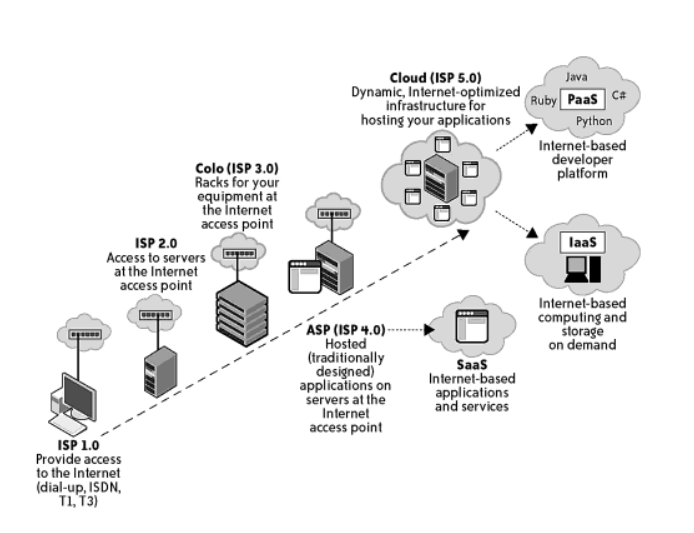
\includegraphics[width=4in]{chapters/chapter2/fig/ISP.PNG}
\caption{Evolution of Cloud Computing from  \cite[p.4]{CloudSec}}
\label{fig_ISPEVO}
\end{figure}

Mather et al.  \cite{CloudSec} describe the emergence of cloud computing as a logical evolution of computing itself and view it as a development of the internet service providers (ISP). Figure \ref{fig_ISPEVO} shows the evolution towards cloud computing.
At first ISPs merely provided Internet access to their customers (ISP 1.0). After the access to the Internet became common, ISPs extended their offerings towards providing additional services like email and access to the servers at their facilities (ISP 2.0). This led to so-called collocation facilities (ISP 3.0), data centers where the ISP provided the infrastructure for the customer servers to be hosted. The next step in the evolution was the application service provider (ASPs), which added additional higher services like customized application for organizations (ISP 4.0). The service delivery model of ASPs may appear very similar to cloud computing, especially to the Software as a Service (SaaS) model, but there is a key difference in the underlying infrastructure. Within the ASP model every customer had his own dedicated infrastructure, so therefore every customer even had his own dedicated server and sole access to it. While cloud computing (ISP 5.0) offers access to shared resources.

As predicted by the Gartner Research Group  \cite{Gartner}, cloud computing is moving towards productivity and establishing itself as new means of getting IT resources and computational power. Figure \ref{Hype} shows the Technology Hype Cycle for 2014, where it can be seen that after the initial peak interest and the following disillusionment cloud computing was expected to reach maturity and the plateau of productivity within the  2 to 5 years. In 2018 the Gartner Research published an standalone hype cycle for cloud computing  \cite{gartnercc18}. This can be seen as a strong indicator of the increasing importance of cloud computing. In Germany, according to the german Association for Information Technology, Telecommunications and New Media (BITKOM)  \cite{BITKOM}, in 2013 40\% of all german companies were using cloud services. In 2018 this number has risen to 73\%  \cite{BITKOM19}. Especially large companies with over 2.000 employees increasingly rely on this technology. Overall cloud computing is immensely popular. Juniper Research  \cite{Juniper} estimated the overall global cloud service users in 2013 to be 2.4 billion. Cloud computing is therefore a focal point for researchers in computer science.

\begin{figure}
\begin{minipage}[hbt]{7cm}
	\centering
	\includegraphics[width=7cm]{chapters/chapter2/fig/Hypeex.PNG}
	\caption{Hype Cycle Phases}
	\label{Hypeex}
\end{minipage}
\hfill
\begin{minipage}[hbt]{8cm}
	\centering
	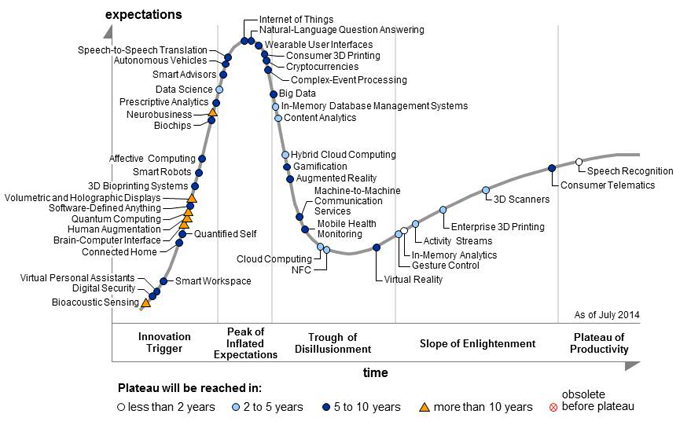
\includegraphics[width=8cm]{chapters/chapter2/fig/hype.jpg}
	\caption{Gartner Group Technology Hype Cycle 2014  \cite{Gartner}}
	\label{Hype}
\end{minipage}
\end{figure}


\begin{figure}
		\centering
		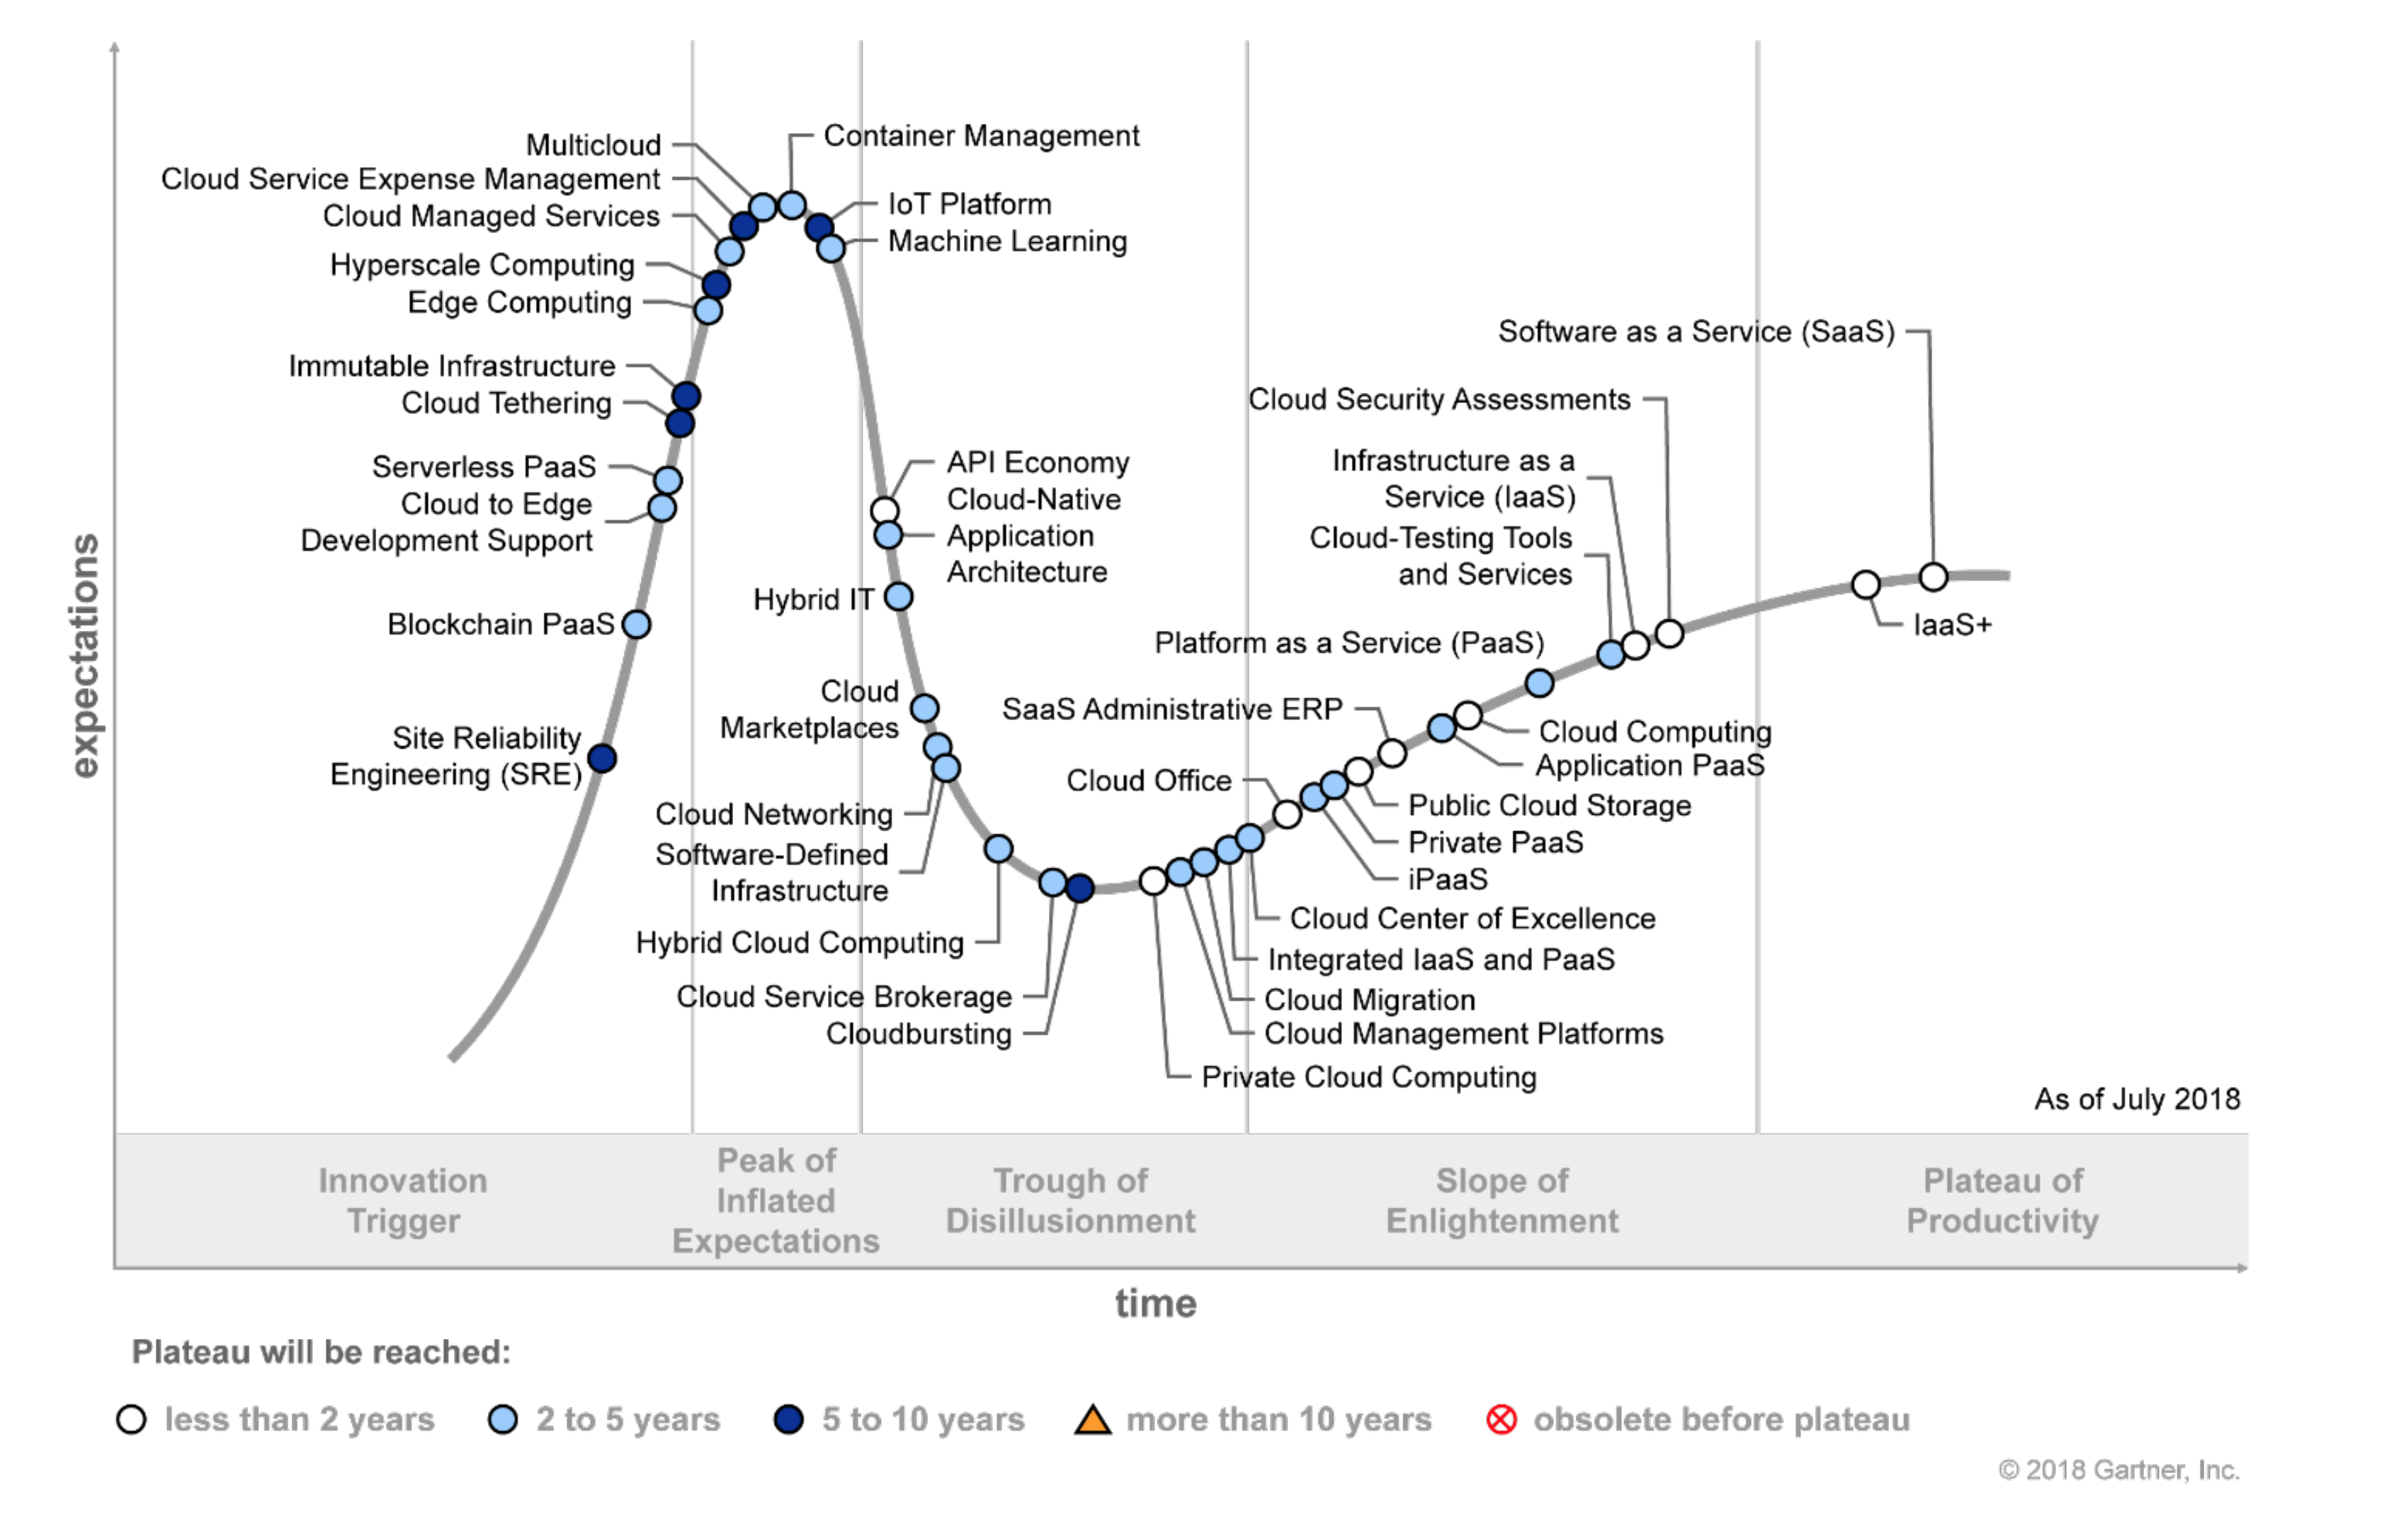
\includegraphics[width=8cm]{chapters/chapter2/fig/hype2.png}
		\caption{Gartner Group Cloud Hype Cycle 2018  \cite{gartnercc18}}
		\label{Hype2}
\end{figure}




\subsection{Cloud Computing Definition}
Even though cloud computing has become very popular in recent years, it is still difficult to get a generally accepted definition of it. What come closest to that is the definition of the US National Institute of Standards and Technology (NIST), which presents itself as a de facto standard for cloud computing:

\textit{"Cloud Computing is a model for enabling convenient, on-demand network access to a shared pool of configurable computing resources (e.g., networks, servers, storage, applications and services) that can be rapidly provisioned and released with minimal management effort or service provider interaction. This cloud model promotes availability and is composed of five essential characteristics, three service models and four deployment models"} NIST Definition of Cloud Computing  \cite{NIST}\\

\begin{figure}[!ht]
\centering
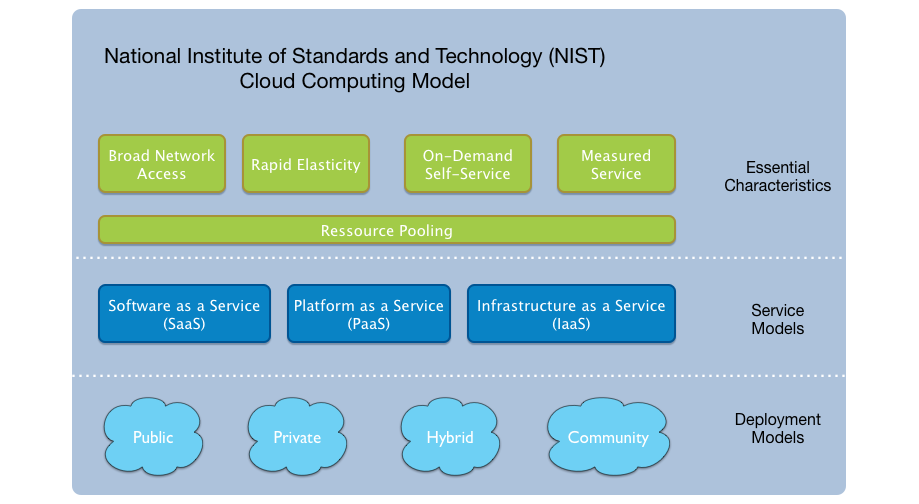
\includegraphics[width=6in]{chapters/chapter2/fig/NIST.PNG}
\caption{NIST Cloud Computing Model  cf.  \cite{NIST}}
\label{fig_NIST}
\end{figure}

A graphical representation of the cloud model based on the definition from NIST is shown in Figure \ref{fig_NIST}. Here all the essential characteristics, service models and deployment models can be seen at once.


\subsection*{Characteristics }
The NIST cloud computing definition identifies the following five essential cloud characteristics:

\textbf{\textit{On-demand self service:}} Cloud customer can provision and manage cloud resources like computing power and network storage without requiring human interaction with a service provider.

\textbf{\textit{Broad network access:}} Provided resources are accessed via networks (mostly the internet) using standardized protocols.

\textbf{\textit{Resource pooling:}}The computing and storage resources of a provider are shared between multiple customers (multi-tenant model). A customer doesn't know the exact physical location of the resources he is using, but may specify a location on an higher abstraction level.

\textbf{\textit{Rapid elasticity:}} Resources can be provided elastically and scaled rapidly to fulfill the customers current demand. This can also be done automatically.

\textbf{\textit{Measured service:}}Consumption of resources by the customer gets metered. The cloud customer only pays for the  resources and services he actually used. For transparency usage is controlled, monitored and reported to both provider and customer.

\subsection{Cloud Models}
As seen in Figure \ref{fig_NIST} another distinction is made between the three service models Infrastructure as a Service (IaaS), Platform as a Service (PaaS) and Software as a Service (SaaS). Figure \ref{fig_CloudPyramid} below shows the differences between the service models regarding flexibility and provider management. 

\begin{figure}[!ht]
\centering
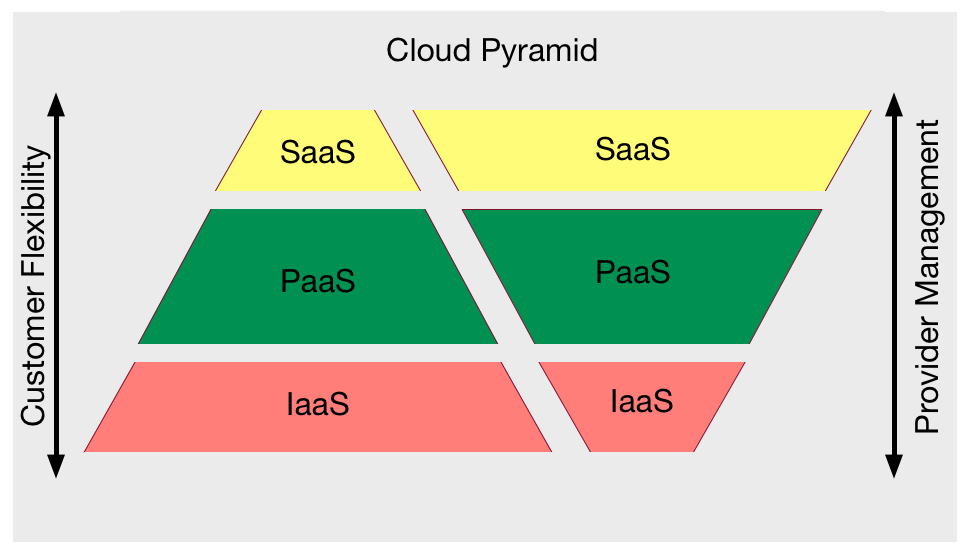
\includegraphics[width=4in]{chapters/chapter2/fig/CloudPyramid.PNG}
\caption{Cloud Pyramid of Flexibility and Management}
\label{fig_CloudPyramid}
\end{figure}

It becomes evident that the models with increased flexibility in terms of usage come with less provider management and involvement, which means that the customer has to manage them by himself. This gets particularly clear with the Infrastructure as a Service model.

\textbf{Infrastructure as a Service (IaaS)} \\
Within the IaaS service model typical infrastructure components like virtual machines, CPU power, memory, storage and networking is provided. The user is able to run and deploy software on this resources at will. This may include operating systems. For this the physical infrastructure of the provider is virtualized by technologies like KVM, Xen or VMware and orchestrated into the virtual infrastructure for the user. The user does not control or manage the physical cloud infrastructure but can control and manage the virtual instance together with the operating system and the components that form the virtual instance, for example host-firewalls, load-balancer and so on. The main difference to traditional hosting servicer like server homing, is that the user only is provided with a virtual instance instead of the physical hardware. For cloud providers this means that they can better divide their resources between customers and so boost overall utilization. The provider charges the customer based on the amount and time of resources he has used on a on-demand model. The provider is responsible for the availability and usability of the infrastructure. Everything else like the reasonable usage, configuration and installation, as well as integration into the  customers IT landscape and connection to other system remains with the customer. Often providers offer automatic installation services for operating systems based on virtual machine images. This may require based on the software additional licensing cost but mostly is offered as a free service. Storage as a Service is a IaaS model where only access to disk space is granted. This model  become increasingly popular in recent years, since it also enables users to easily share their data with third parties. Best known for this are providers like Dropbox  \cite{Dropbox}, Microsofts OneDrive  \cite{OneDrive} or Google Drive  \cite{GoogleDrive}. Most popular IaaS providers at the moment are Amazon Web Services  \cite{AWS} and Rackspace  \cite{rackspace}. Lately Google Compute Engine  \cite{Googlecompute} and  Microsoft Windows Azure  \cite{Azure} started their IaaS services.\\

\textbf{Platform as a Service (PaaS)}\\
This model aims at developers by providing comprehensive development and run environments to easily create, test and deploy applications. The user gets presented with a pre-configured environment by the provider, which means he does not have to deal with management or install of the virtualized infrastructure. The provider defines and configures as well all the development tool kits and environments, programming languages, APIs. libraries and databases. In extensive PaaS  offerings users can immediately start to develop or deploy applications,  without even installing  tools on their machines. This model therefore enables developers a rapid propagation of their applications, location independent multi-tenant development and minimal entry effort and cost. Well known PaaS offers are Google App Engine  \cite{GoogleAppEngine} and Microsoft Windows Azure  \cite{Azure}.\\

\textbf{Software as a Service (SaaS)}\\
In the SaaS model the user is provided with the capability to use the applications running on the providers cloud infrastructure. The users does neither manage, nor control the infrastructure or its components, the operations system or any application capabilities with the exception of settings within the applications. The user usually accesses the rented applications through either the web browser or an adapted program interface. In contrast to traditional software usage the customer subscribes to the service or uses a pay-per-use model. It is quite common that SaaS provider use PaaS or IaaS infrastructures or third party providers to benefit form the high elasticity. Popular SaaS providers are Google Apps  \cite{GoogleApps}, Google Docs  \cite{GoogleDocs}, Microsoft Office 365  \cite{Office365} and Salesforce.com  \cite{Salesforce}.




\subsection*{Deployment Models}
The NIST definition identifies four different deployment models. As seen in Figure \ref{fig_NIST} these are: Public cloud, Private cloud, Hybrid cloud and Community cloud.  

\textbf{Private clouds} are used exclusively by one single organization, for example by a company for serving its internal needs. These cloud are also often referred to as internal clouds, since the infrastructure is commonly run inside the private network of the using entity. The cloud system may be operated and managed by the organization itself, a third party or a combination of both.\\

\textbf{Public clouds} represent the exact opposite. Here the usage of the cloud is not limited to one user respectively one organization, instead the services are offered to a larger group of customers or the general public. This cloud type is also called external clouds, since they are managed, hosted and operated by a third-party vendor outside the influence of the customer. The services are commonly accessible through web-applications, web-services or communications protocols like the Remote Desktop Protocol (RDP) or Secure Shell (SSH). A well known provider for public cloud services is the Amazon Elastic Compute Cloud (EC2).\\

\textbf{Community clouds} are used exclusively  by a specific community of consumers. This usually are organizations that have shared concerns (e.g., mission, security requirements, policy, and compliance considerations cf.  \cite{NIST}). The infrastructure my exist on or off premises, as well as may be owned, operated and managed by one or more of the community entities or a third party or any combination of the mentioned before.\\

\textbf{Hybrid clouds} present a composition of two or more of the mentioned above cloud deployment models. The infrastructures are bound together but still remain unique entities. This is done by enabling data and application portability through the use of standardized or proprietary technology.

\subsection{Reference Architecture}
Different cloud architectures include various components. In terms of a wide acceptance the NIST proposed architecture is chosen to give an overview of possible components. The NIST architecture identifies  five major actors. Table \ref{tab_NISTArchAct} shows these actors and gives the definition of them. The descriptions are taken directly from the  NIST Cloud Computing Reference Architecture  \cite{NISTArch}.\\

\begin{table}[h]
    \begin{tabular}{| l|p{11cm} |}
    \hline
    \textbf{Actor }          & \textbf{Definition   }                                                                                                                                           \\ \hline
    Cloud Consumer  & A person or organization that maintains a business relationship with, and uses service from, Cloud Providers.                                           \\ \hline
    Cloud Provider  &  A person, organization, or entity responsible for making a service available to interested parties.                                                    \\ \hline
    Cloud Auditor   & A party that can conduct independent assessment of cloud services, information system operations, performance and security of the cloud implementation. \\ \hline
    Cloud Broker    & An entity that manages the use, performance and delivery of cloud services, and negotiates relationships between Cloud Providers and Cloud Consumers.   \\ \hline
    Cloud Carrier   & An intermediary that provides connectivity and transport of cloud services from Cloud Providers to Cloud Consumers.                                     \\ \hline
    \end{tabular}
    \caption {Cloud Computing Actors from NIST  \cite{NISTArch}}
    \label{tab_NISTArchAct}
\end{table}

The Cloud Provider is the entity that delivers the cloud service to the Cloud Consumer. Since the delivered service are to be consumed over a broad network access a third party. the Cloud Carrier is used to provide connectivity between the both. This can for example be the Internet Service Provider or in case of a private cloud it would be the IT department responsible for the network. In some cases different roles can be adopted by one organization this may be the case especially with private clouds but also if the Cloud Provider at the same time is a ISP and therefore takes the role of the Cloud Carrier.

A Cloud Provider usually owns one ore more different data centers (facilities).  Here the physical hardware for  the cloud infrastructures and the environment needed (cooling, electric power, ...) to support it is hosted. In the presented architecture this is grouped together as the \textit{physical resource layer}. Figure \ref{fig_NISTArch} shows the overview of the components of the NIST cloud architecture. 

In between the \textit{physical resource layer} and the \textit{service layer}, which provides the three different service model (IaaS, PaaS, SaaS) there is the \textit{resource abstraction and control layer}.  These three layers form the \textit{Service Orchestration} module which is used to compose and deliver the actual cloud services. The \textit{service layer }on top is where the Cloud Provider defines the access interfaces for the Cloud Consumer. In the course of this it is possible but not necessary that SaaS applications can be built on top of PaaS components and these again can be built on top of IaaS components. So for example, a PaaS environment could be hosted on top of a virtual machine from an IaaS cloud.

The \textit{resource abstraction and control layer }contains all system and software components that the Cloud Providers uses to abstract the physical resources into virtualized cloud resources. This may include hypervisors or virtual machine monitors, virtual storage, virtual machines and so on. The virtualization in this layer allows resource pooling, dynamic allocation and measurement of the consumed services. Here the control (allocation, access control and usage monitoring) of the cloud resources is realized.

\begin{figure}[!ht]
\centering
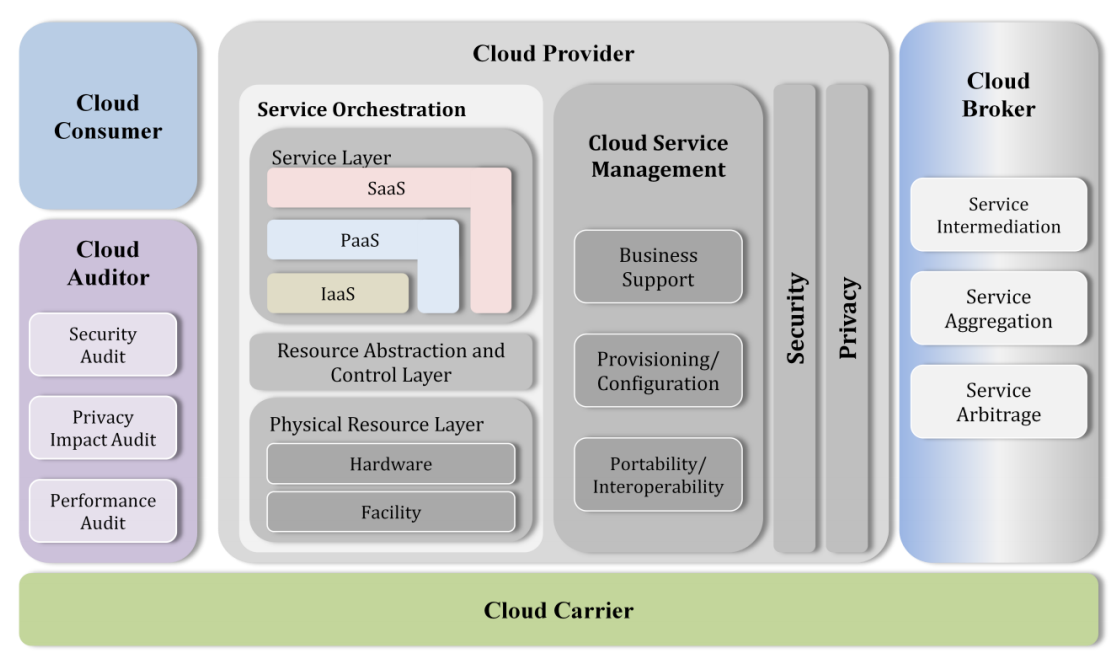
\includegraphics[width=6in]{chapters/chapter2/fig/RefArch.PNG}
\caption{Cloud Computing Reference Architecture from NIST  \cite{NISTArch}}
\label{fig_NISTArch}
\end{figure}

In addition to this core component, there is the \textit{cloud service management} and modules for \textit{security} and \textit{privacy}. The cloud service management module includes the functions which are needed by the Cloud Provider for the management and operation of the provided cloud services. These are grouped into three different Cloud Provider perspectives. Firstly the \textit{business support}, which includes the processes supporting the service offering and dealing with clients, like the customer management, contact management, accounting \& billing and reporting \& auditing. Then there are the processes involved in the \textit{provisioning and configuration} of the cloud services. These include the monitoring and metering as well as the SLA management. Lastly there are the mechanisms to support \textit{portability and interoperability}, which shall enable the service customer to freely merge and compose cloud services between different cloud providers. A detailed description of all these three modules and their individual components can be found in the NIST publication  \cite[p. 15]{NISTArch}.

\subsection*{Related Technologies to Cloud Computing}
As described earlier cloud computing has evolved from technologies that date back early in the history of computer science.Therefore it is related to different technologies by sharing similar aspects. Following the shared aspects with virtualization, grid computing, utility computing and autonomic computing  will be shown.

\textbf{Virtualization} presents itself as one of the core technologies of cloud computing. Virtualization abstracts layers of physical resources from one another, thus making it possible to compose virtual systems out of virtual resources. Through aggregation of large computational resources across multiple physical machines, virtual resources can be pooled by the provider. Therefore virtualization forms the foundation of cloud computing, as it provides the capability of assigning and reassigning virtual resources dynamically to cloud customers on-demand  \cite{CloudChallenges}.

\textbf{Grid Computing} aims at creating supercomputer like computing resources by coordinating and utilizing distributed network connected resources. Grid computing initially was driven by scientific applications like protein folding  \cite{Folding@Home} or particle simulation  \cite{ATLAS@Home} or the search for pulsars  \cite{Einstein@Home}. Grid computing always serve a specific task and all participating resources aim to achieve this common objective. Cloud computing appears very similar and shares a lot of the attributes from grid computing, for example the use of distributed resources and abstracted utilization. But it differs in term of dynamic resource provisioning, the abstractions, the business model and applications  \cite{Cloud360}.

\textbf{Utility Computing}  contains the business model of "pay-per-use" for computing services. Much like for example electricity the  provided computing services are metered and the customer is billed based on his usage. Cloud Computing adopts this billing model and therefore can be seen as a realization of utility computing.

\textbf{Autonomic Computing} was coined by IBM in the early 2000s, where autonomic refers to self-managing computer systems. The aim was to create computing systems that were able to react and respond to internal and external observations without any human interaction. Cloud computing shares some of the aspects considering self-management, like autonomic provisioning of resources with autonomic computing. But instead of aiming for fully autonomous systems with for example self-correction the aim in cloud computing is to reduce management involvement and improve the on demand character.


\subsection{Cloud Computing Advantages and Disadvantages}
Cloud computing comes with many benefits especially for small and medium sized business users. In this section the advantages are described both form perspective of the provider and consumer. As one of the major benefits of cloud computing the increased agility and adaptability can be seen. Here customers can take advantage of extending their IT capabilities based on the demand to fit the changing requirements. In addition the customer does not have to manage or maintain the underlying infrastructure, which reduces his personnel training efforts and costs and therefore can stronger focus on his core strengths. Cloud computing also makes it possible to obtain enormous computing resources within very short times without having to bear the cost of acquisition. Due to this low up-front investments cloud computing offers a low entry barrier for young companies and simultaneously enabling rapid testing and development. For cloud providers using the virtualization technologies enables them to better utilize their infrastructure, by dividing the distributed physical hardware into virtual resources, since not all of the services in usually use the full provided resources. This reduces the overall Total Cost of Ownership (TCO). Because providing cloud services is the core competence of the cloud provider the offered services usually provide better performance and availability. Especially for SMEs it would be very expensive to reach the same high availability levels of modern cloud computing providers and depending on the usage cloud computing reduces the operating and maintenance cost of the customers services  \cite{CCbasics}. This is due to the on-demand character of the cloud where the customer can reduce the rented resources of his  services with low usage to a minimum. This reduces costs for the customer, while he still is being able to quickly adapt them back in case of increasing demand so that business risks of under-performance is reduced. In addition the further risks like recovery due to outage or hardware failure is also moved to the cloud provider.

Besides the aforementioned benefits cloud computing also bears some disadvantages and risks. The main concern of many cloud users still is security  \cite{CloudConcerns}. The primary concern for many users is the loss of control over data or the infrastructure ( \cite{6409059},  \cite{Zissis2012583}). This is due to lack of a proper, cloud provider  independent security model. In addition the often unknown physical location of the rented resources (especially in public clouds) and the absence of cloud security standards and improper backups bare a risk of data loss. Besides that the use of cloud computing does not always mean a reduction in operational costs. For permanent use classic hosting offerings are significantly cheaper. For example a streaming server based on a t3a.xlarge Amazon EC2 instance with 4 vCPU cores (AMD EPYC processors with an all core turbo clock speed of up to 2.5 GHz), 16GB memory, 500GB SSD, located in Frankfurt would costs around 140 USD  \cite{AWSprice}. In contrast a conventional dedicated hosted server with  2x Intel Xeon E5 2.1+ GHz CPU, 16 GB of memory, 2x 1000GB RAID, with a 1 Gbit/s connection and unlimited traffic, would cost about 260 EUR  \cite{Contabo}. Additionally all cloud services are heavily network dependent, respectively Internet dependent. So the availability and performance of the connection is a core requirement for using cloud services. In case of missing or bad performing connections the provider is not necessarily responsible, since he only has to provide his services towards his edge of the network, so users have to ensue reliable connections. A additional risk may be the dependency on the vendor and possible vendor lock-in. This occurs due to the lack of interoperability between cloud providers. Virtualization adds abstraction between the users and the physical hardware, but since not all virtualization technologies are inter operable moving from one cloud provider to another may be difficult. 


\section{Service Level Agreements}
A service level agreement (SLA) in general is a formal bilateral legal contract between a provider of services and the consumer of such services, that defines the scope and quality expected that the provider commits to deliver to the customer. The Information Technology Infrastructure Library defines SLA as the following:

\textit{Service Level Agreement- A formal, negotiated document that defines (or attempts to define) in quantitative (and perhaps qualitative) terms the service being offered to a Customer. Confusion must be avoided over whether the quantitative definitions constitute thresholds for an acceptable service, targets to which the supplier should aspire or expectations that the supplier would strive to exceed. Any metrics included in a Service Level Agreement (SLA) should be capable of being measured on a regular basis and the SLA should record by whom. } ITIL V2  \cite{ITILweb}

The aim of such contracts is create a reliable, legally binding arrangement from witch both the customer and the provider can benefit. The content of a SLA will typically will cover general service related information like service hours and availability, but also will include the performance expectations and desired service outcomes in term of functionality and responsiveness. This also may include incurring costs, information about security and additional terminology. For customers it offers the possibility to guarantee their expected service outcome and in case of non-compliance enable financial compensation. For providers it states clearly all the agreed upon deliverables, as well as the method of delivery, occurring costs, verification and sanctions he has to comply to. So that he can deliver his services based on that and charge the customer without any discrepancies. The other side of the coin is the provider needs to establish SLA management so that he can satisfy the contracts. 

Since Service Level Agreements specify the promised respectively the expected performance characteristics of a service, the most important part is the exact description of the service quality (service level). But the creation of Service Level Agreements provides requirements to customers and providers. Customers need to be able to meet certain requirements in order to successfully define SLAs, which are listed briefly below  \cite{SLAEntwurf}.

 A customer must:
\begin{itemize}
\item Understand the roles and responsibilities that are regulated by the SLA.
\item Be able to describe precisely and specific the service  to be controlled by the SLA.
\item Know the requirements of the controlled services, and define the matching key figures.
\item Specify service levels based on the critical performance characteristics of the service.
\item Understand the process and procedures of regulated service.
\end{itemize}

These requirements are necessary so that the customer is able to put in the correct SLAs values, and to understand implications of his decisions. Furthermore, a SLA should fulfill the following tasks:
\begin{itemize}
\item Describe the services accurately.
\item Specify the service quality to be provided in detail.
\item Describe detailed the key performance indicators, metrics and service levels.
\item Breakdown transparently all the costs.
\end{itemize}


\subsection{SLA Life Cycle}
The life cycle of a service level agreement involves several steps for a successful use of SLAs \cite{sun2005role}. There are different views on whether  the negotiation phase of the SLA is one of its life cycle or not, since this can also be counted among the preconditions (cf.  \cite{hasselmeyer2007negotiating} and  \cite{gangadharan2007service}).  Figure \ref{fig:SLA_Lifecycle} shows the SLA life cycle from  \cite{scholderer2011management}.

\begin{figure}[ht]
\begin{center}
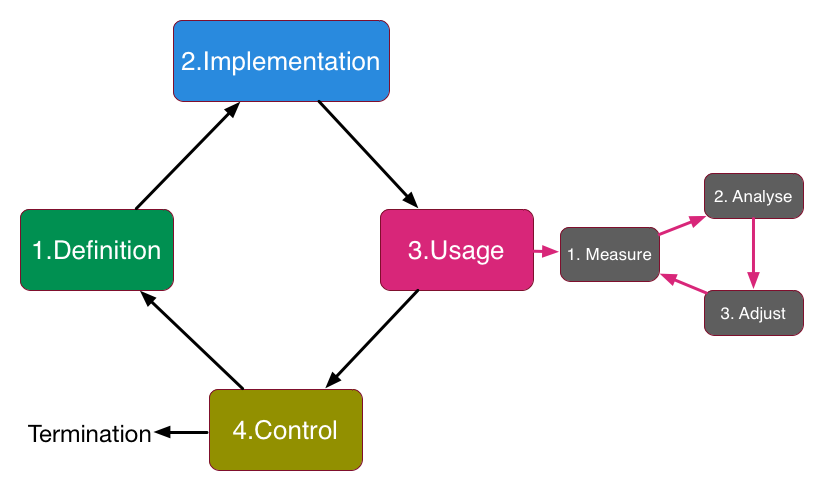
\includegraphics[width=0.7\textwidth]{chapters/chapter2/fig/SLAMlifecycle.png}
\caption{SLA Life Cycle}
\label{fig:SLA_Lifecycle}
\end{center}
\end{figure}

The preconditions for this life cycle is that the negotiation phase is integrated within the definition, where the deliverable  service levels and the costs are negotiated with the provider. This negotiation process usually includes several rounds of proposals and definitions of services. After it is done, the agreed upon binding SLA is created and signed by both parties. While in the implementation phase, the validity of the agreement is marked by the signatures of both partners. Here the provided services are provisioned and the agreements are communicated  and fitted into the organizations. During the usage phase the customer uses the service according to his notions. Parallel to this, the service performance is monitored during runtime and assessed against the service levels. If needed, corrective actions are executed and reports and documentation are created for the partners. The final control phase marks either the end of the usage by the customer, if they no longer needs or wants to use the service, which initiates the decommission of the service. Otherwise the SLA is checked against the altered requirements and then a new definition process is started.

\subsection{SLA Content}
The structure of service level agreements are generally very scenario specific and can not be easily generalized. However, there are some basic elements that should be present in every SLA. The following remarks are not intended to be used to create an universal pattern for SLAs, but rather give a outline for most current contents of SLAs. The contents of a SLAs can be generally divided into the following four categories: (see  \cite{Berger05}) \textit{agreement-related elements, service-related elements, document-related elements and\\ management-related elements.} 
 
The \textbf{agreement-related elements} contain the basic rules of the agreement and include, among others, the subject of SLAs, objectives, partners, as well as the scope, entry into force, duration and termination of SLAs. Often these elements are shown in practice in the form of a preamble or introduction. The subject of SLAs introduction here describes the content and context as well as a description and demarcation of the services being controlled by the SLA.The objectives of the SLAs reflect the specific objectives of both parties and serve, among other things, as a basis for future success control. 
 
The \textbf{service-related elements} represent those elements which describe the regulation of a service. These must be specified individually for each service. The content is basically to describe who, when, where, and what services are provided. The description of the service should be generally understandable. The description of the quality of a service is the central role of the SLA. The negotiated quality of service is often represented by technical Key Performance Indicators (KPIs), which form the basis for the Service Level Objectives" (SLOs). These indicators include a label next to the calculation or metric, and a reference area and measurement point. KPIs also often target organizational  objectives of the service provider and not only technical aspects. It should be noted that not every metric automatically relates to a Key Performance Indicator. KPIs are bound to organizational or services goals and must aim towards attainability.

\begin{figure}[ht]
\begin{center}
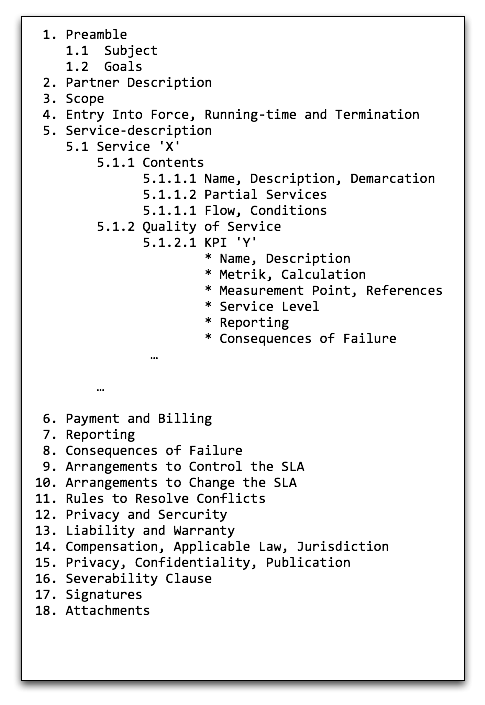
\includegraphics[width=0.5\textwidth]{chapters/chapter2/fig/content.png}
\end{center}
\caption{SLA Structure}
\label{fig:SLA_Structurex123}
\end{figure}

 
\textbf{Document-related elements} include administrative and editorial elements, which play  a minor role inside a SLA and are mainly there to improve the handling, understanding and readability. These elements are, e.g., version, the date of last modification, revision history, table of contents, the index or glossary. These elements increase the readability by underpinning the context and explain the background. 
 
The \textbf{management related elements} include the aspects that have to do with the administration and control of SLAs. These represent a very important section of the contents of a SLA,since both the customer notification and the procedure in case of problems or failures to meet the service levels are regulated. Furthermore, penalties and compensation in case of damage which may occur due to deviations from service levels are regulated. 

Based on the presented elements, a generalized structure of a SLA has been created, which can be seen in Figure \ref{fig:SLA_Structurex123}. Here, it is clear that the service descriptions, or service level objectives form the central aspect of each SLA. These and their contents are described in more detail in the following sections. Likewise, it comes clear that even small SLAs mean large administrative overhead and the creation is a lot of work.


\subsection{Service Level Objectives}\label{section_SLO} 
Service Level Objectives (SLOs) are a central element of every service level agreements (SLA), which include the negotiated service qualities (service level) and the corresponding Key Performance Indicators. SLOs contain the specific and measurable properties of the service, such as availability, throughput or response time and often consist of combined or composed attributes. SLOs should thereby have the following characteristics: cf.  \cite{RW00} 

\begin{itemize} 
\item achievable / attainable 
\item repeatable 
\item measurable 
\item understandable 
\item significant 
\item controllable 
\item affordable 
\item mutually acceptable 
\item influential 
\end{itemize} 

A SLOs should always contain a target value or desired service level, a metric and corresponding measurement period, as well as the type and location of the measurement. For this purpose, usually KPIs with associated service level values are stated. KPIs should contain information about the measurement process, measurement destination and unit as well. A valid SLO specification might, for instance, look like this: \textit{The IT system should achieve an availability of 98\% over the measurement period of one month. The availability represents thereby the ratio of the time in which the service works with a response time of less than 100ms plus the planned downtime to the total service time, measured at the server itself.} From such a description, the actual performance values can be compared with the reference values of the SLOs and the achieved availability result is calculated. Based on this, further measures can be carried out or correction measures can be conducted if necessary. 
 
\section{Conclusion}
In this chapter the historic development and essential attributes of cloud computing were introduced, as well as a definition of cloud computing together with a reference architecture were given. The main cloud  service and deployment models were presented and related technologies were introduced and delimited from cloud computing. Finally the advantages as well as the disadvantages of cloud computing were discussed. Additionally, the essential attributes and contents of service level agreements have been stated as well as a definition based on ITIL V2. The main SLA elements were discussed and the related life cycle was introduced and illustrated. Finally a generalized structure and service level objectives were introduced. Along side with the here introduced self-management respectively autonomous systems , this forms the foundations for the system presented .
